%==============================================================================
%  Auxiliary report: possible worlds, the conflation rate, and the scope of
%  semantic entropy. Companion to the paper "Who Said It?" (paper/main.tex).
%  1o Desafio de Dados do Instituto Kunumi - 2026  (Ideias em Rede, 1a Edicao)
%
%  Compile:  pdflatex -> bibtex -> pdflatex -> pdflatex
%  Every number in this report is printed by a script in code/ (see the
%  Reproducibility section and README.md).
%==============================================================================

\AddToHook{package/amssymb/before}{\let\Bbbk\undefined}
\documentclass[english]{desafiokunumi}

\usepackage{tikz}
\usetikzlibrary{arrows.meta}
\let\openbox\undefined
\usepackage{amsthm}
\usepackage{array}

% The class hard-codes "Resumo."/"Palavras-chave:" even under [english].
\usepackage{etoolbox}
\makeatletter
\patchcmd{\maketitle}{Resumo.}{Abstract.}{}{\typeout{[aviso] rotulo Resumo nao encontrado}}
\patchcmd{\maketitle}{Palavras-chave:}{Keywords:}{}{\typeout{[aviso] rotulo Palavras-chave nao encontrado}}
\makeatother

\newtheorem{proposition}{Proposition}
\newtheorem{observation}[proposition]{Observation}
\theoremstyle{definition}
\newtheorem{definition}[proposition]{Definition}
\theoremstyle{remark}
\newtheorem{remark}[proposition]{Remark}

\newcommand{\SE}{\mathrm{SE}}
\newcommand{\SEc}{\mathrm{SE}_{\mathrm{core}}}
\newcommand{\WE}{\mathrm{WE}}
\newcommand{\Ind}{\mathrm{Ind}}
\newcommand{\cf}{\mathrel{\#}}
\newcommand{\cfz}{\mathrel{\#_0}}

\renewcommand{\arraystretch}{1.05}
\captionsetup{skip=4pt}
% Same spacing adjustments as the main paper (theorem and display skips).
\makeatletter
\def\thm@space@setup{\thm@preskip=4pt \thm@postskip=4pt}
\makeatother
\setlength{\abovedisplayskip}{4pt plus 2pt minus 2pt}
\setlength{\belowdisplayskip}{4pt plus 2pt minus 2pt}
\setlength{\textfloatsep}{10pt plus 2pt minus 2pt}

% =============================================================================
%  METADATA
% =============================================================================
\title{When Does Answer Diversity Mean Disagreement? Possible Worlds and the Scope of Semantic Entropy}
\subtitle{{\normalsize\mdseries Auxiliary report to the paper \emph{Who Said It? Speaker-Conditioned Verification and Lexicographic Tie-Breaking for Low-Cost Hallucination Detection in Legislative Hearings}}}

\authors{%
  Gabriel Ribeiro\textsuperscript{1}, Cau\~a Sathler\textsuperscript{2},
  Arthur Gon\c{c}alves\textsuperscript{1}, Jordan Elias\textsuperscript{3}%
}

\affiliations{%
  \textsuperscript{1}Colab Domain-Specific Foundation Models, Departamento de
  Ci\^encia da Computa\c{c}\~ao, Universidade Federal de Minas Gerais (DCC-UFMG)\\
  \textsuperscript{2}Colab Agentic AutoML for Data Science, Departamento de
  Ci\^encia da Computa\c{c}\~ao, Universidade Federal de Minas Gerais (DCC-UFMG)\\
  \textsuperscript{3}Colab SLMs for Process Automation, Universidade Federal do
  Cear\'a (UFC)\\[2pt]
  \texttt{gabriel.ribeiro@dcc.ufmg.br}, \texttt{cauasathler@ufmg.br},\\
  \texttt{afariag72@gmail.com}, \texttt{jordanelias@alu.ufc.br}%
}

\keywords{semantic entropy; natural language inference; contradiction; possible worlds; event structures; uncertainty quantification; hallucination detection}

\abstracttext{Sampling-based uncertainty methods such as semantic entropy group a model's sampled answers into classes of equivalent meaning and read many classes as a sign that the model does not know the answer. This report, which accompanies our paper on hallucination detection in PublicHearingBR, examines a distinction these methods do not make: two answers can differ because they contradict each other or because both can be true. Using the contradiction probabilities that the natural language inference model already computes, we represent an answer set as an event structure whose maximal consistent subsets, its possible worlds, can be enumerated exactly. We show that semantic entropy and every quantity derived from the entailment order are blind to this distinction, and we measure it in three settings. On TriviaQA, the model's answer is correct $81\%$ of the time when its samples share one meaning, $44\%$ when they differ but fit in a single world ($n=18$) and $22\%$ when they span several worlds ($n=125$), although the last two rates do not differ significantly. The share of multi-class answer sets that form a single world, which we call the conflation rate, is $12.6\%$ in short-answer question answering and $78.5\%$ in closed-book statements about hearings. Asking the same TriviaQA questions for full-sentence answers raises the conflation rate to $29.0\%$ and lowers the AUROC of semantic entropy from $0.816$ to $0.721$ (paired difference $-0.095$, $95\%$ CI $[-0.175,-0.016]$). Entropy over worlds does not outperform semantic entropy where the latter works, and consistency features do not detect hallucinations in PublicHearingBR; we report both negative results in full.}

\begin{document}
\raggedbottom
\maketitle

% =============================================================================
\section{Introduction}
\label{sec:intro}

This report accompanies the paper \emph{Who Said It? Speaker-Conditioned
Verification and Lexicographic Tie-Breaking for Low-Cost Hallucination
Detection in Legislative Hearings}, submitted to the first data challenge of
Instituto Kunumi. The paper checks opinions attributed to participants of
legislative hearings against the attributed speaker's own turns and combines
inexpensive detectors with a committee of LLM judges. A second line of our
project studied a different question, which the paper leaves out for reasons
of space and scope: when a language model's sampled answers differ, how much of
the difference is disagreement? This report presents that study, including
its negative results. It can be read independently of the paper;
Section~\ref{sec:neg} contains the one result the paper cites.

A common way to estimate whether a language model knows an answer is to sample
it several times and measure how much the samples differ
\citep{manakul2023selfcheckgpt,kuhn2023semantic}. \emph{Semantic entropy}
\citep{kuhn2023semantic,farquhar2024semantic} groups the samples into classes
of answers that entail each other, according to a natural language inference
(NLI) model, and computes the entropy of the class frequencies. One class means
that the samples agree; many classes are read as a sign that the model does not
know. On short-answer question answering this works well: on TriviaQA
\citep{joshi2017triviaqa}, semantic entropy reaches an AUROC of $0.811$ in our
setup (Section~\ref{sec:res-p3}).

Two answers can fall into different classes for three reasons. They can
contradict each other (``the committee approved the bill'' and ``the committee
rejected the bill''); one can refine the other (``the committee approved the
bill by a wide margin''); or they can state different facts that are both true
(``the session lasted four hours''). Only the first is a disagreement about
what happened. Semantic entropy counts all three alike, although the NLI model
it already runs returns a contradiction probability for every pair of answers.
Methods that do use contradiction treat it as a score, such as an average or a
density (Section~\ref{sec:bg-related}), rather than as a constraint on which
answers can be true together.

We use that constraint directly. Section~\ref{sec:worlds} represents an answer
set as an event structure \citep{winskel1987event}: answers ordered by
entailment and related by conflict. Its maximal consistent subsets, which we
call \emph{worlds}, are the complete accounts the samples support, and they can
be enumerated exactly. Section~\ref{sec:blind} shows that semantic entropy and
every quantity computed from the entailment order are blind to conflict, and
Sections~\ref{sec:dados}--\ref{sec:neg} measure what this blindness costs. Our
contributions are:
\begin{itemize}\setlength{\itemsep}{1pt}
  \item a formal account of which answers can hold together
  (Proposition~\ref{prop:mundos}), with an entropy over worlds that needs no
  model calls beyond the NLI passes semantic entropy already makes;
  \item evidence that conflict carries information the entailment order does
  not: on TriviaQA, $97.9\%$ of conflicts join classes the order does not
  compare, and the accuracy of the model's answer falls from $81.1\%$ (one
  class) to $44.4\%$ (several classes in one world, $n = 18$) and $22.4\%$
  (several worlds), although the last step is not significant;
  \item the \emph{conflation rate}, a statistic computed without labels, which
  is $12.6\%$ on TriviaQA and $49.3$--$78.5\%$ for closed-book statements about
  hearings, together with an intervention on the same TriviaQA questions in
  which a higher conflation rate comes with a significant drop in the AUROC of
  semantic entropy;
  \item negative results: the entropy over worlds does not outperform semantic
  entropy where the latter works; in PublicHearingBR, contradictions among the
  retrieved evidence carry no detectable information about hallucination beyond
  the amount of evidence; and none of the self-consistency quantities we
  tested, ours included, detects answers built on misleading evidence.
\end{itemize}
All predictions were written to the repository before the corresponding
measurement (Section~\ref{sec:pred}). Results outside the registered
confirmatory comparisons are labelled exploratory.

% =============================================================================
\section{Background}
\label{sec:bg}

\subsection{Natural language inference}
\label{sec:bg-nli}

An NLI model reads an ordered pair of sentences, a premise and a hypothesis,
and returns three probabilities that sum to one (Table~\ref{tab:nli}).
Entailment is directed: ``it was in 1988'' entails ``it was in the 1980s'', but
not conversely. Contradiction is symmetric in meaning, although the model's
estimates for the two orders of a pair can differ. Throughout this report we
use the multilingual checkpoint
\texttt{mDeBERTa-v3-base-xnli-multilingual-nli-2mil7} \citep{laurer2024less}, with a threshold of $0.5$ for both entailment and
contradiction, fixed before any measurement.

\begin{table}[ht]
  \centering
  \caption{The three outputs of an NLI model.}
  \label{tab:nli}
  \small
  \begin{tabular}{@{}lll@{}}
    \toprule
    \textbf{Label} & \textbf{Meaning} & \textbf{Example (premise $\to$ hypothesis)} \\
    \midrule
    entailment    & the premise makes the hypothesis true & ``it was in 1988'' $\to$ ``it was in the 1980s'' \\
    contradiction & the two cannot both be true            & ``it was in 1988'' $\to$ ``it was in 1995'' \\
    neutral       & neither of the above                   & ``it was in 1988'' $\to$ ``it rained that day'' \\
    \bottomrule
  \end{tabular}
\end{table}

\subsection{Semantic entropy and the entailment order}
\label{sec:bg-se}

Consider $N$ answers sampled for the same prompt. Write $a \sqsubseteq b$ when
$a$ entails $b$ with probability at least $0.5$, closed under transitivity
(the NLI model is not transitive by itself). Answers that entail each other
form a \emph{semantic class}, and the mass $p(u)$ of class $u$ is the fraction
of samples in it. \textbf{Semantic entropy} is
$\SE = -\sum_u p(u)\log p(u)$, the discrete estimator of
\citet{farquhar2024semantic}. It is $0$ when all samples share one meaning and
$\log N$ when no two do.

Entailments in one direction only survive the grouping and order the classes:
$u \sqsubseteq v$ means that $u$ entails $v$, so $v$ is the more general
class. A \emph{chain} is a set of classes stacked one above the other, such as
``in 1988'' $\sqsubseteq$ ``in the 1980s'' $\sqsubseteq$ ``in the 20th
century'': one belief at three levels of detail. An \emph{antichain} is a set of
classes no two of which are comparable. Semantic entropy ignores the order: the
chain above and three unrelated answers both give $\log 3$.

As an order-aware comparator we also report the \textbf{core entropy} $\SEc$,
which we developed earlier in this project. A class is \emph{redundant} (a
\emph{beat point}, \citealp{stong1966finite}) if the classes strictly below it
have a greatest element or the classes strictly above it have a least element.
Removing redundant classes one at a time, and moving the mass of each removed
class to the class that witnessed its removal, ends in the \emph{core} of the
order, which is unique up to isomorphism \citep{stong1966finite}. $\SEc$ is the
entropy of the core's masses, averaged over eight removal orders because the
final masses, unlike the core, can depend on the order. On a chain the core is
a single class and $\SEc = 0$; on an antichain nothing is removed and
$\SEc = \SE$.

\subsection{How contradiction is used elsewhere}
\label{sec:bg-related}

SelfCheckGPT \citep{manakul2023selfcheckgpt} can score a sentence by the
average probability that sampled passages contradict it. Kernel language
entropy \citep{nikitin2024kernel} replaces hard classes by a similarity kernel
built from NLI outputs; directional entailment graphs
\citep{da2024directional} keep the direction of entailment; and logical graphs
\citep{lgu2026logical} combine the entailment structure with a scalar density
of contradictions. In these methods contradiction enters as a number (an
average, a weight or a density). To our knowledge, none of them uses it to
determine which answers can be true together, which is the object of this
report.

% =============================================================================
\section{Worlds}
\label{sec:worlds}

This section defines which subsets of an answer set can be held together, first
informally and then formally. Throughout, $P$ is the set of semantic classes of
one answer set, ordered by $\sqsubseteq$, with masses $p$.

\subsection{Conflict and its inheritance}
\label{sec:conflict}

Two classes $u$ and $v$ are in \emph{raw conflict}, written $u \cfz v$, if
some answer of $u$ and some answer of $v$ contradict each other with
probability at least $0.5$, in either order. Contradictions between answers of
the same class are ignored. Raw conflict needs one correction. If ``the
committee approved the bill'' contradicts ``the committee rejected the bill'',
then ``the committee approved the bill by a wide margin'' contradicts it as
well, since anyone who asserts the refinement also asserts what it entails. The
NLI model may miss such inherited contradictions, so we add them.

\begin{definition}[Inherited conflict]
\label{def:closure}
Classes $u$ and $w$ are in \emph{conflict}, written $u \cf w$, if they have
generalisations in raw conflict: $u \sqsubseteq v$, $w \sqsubseteq v'$ and
$v \cfz v'$ for some classes $v, v'$, where every class counts as a
generalisation of itself. If $P$ and $C_0$ denote the Boolean matrices of
$\sqsubseteq$ and $\cfz$, the conflict matrix is
$C^* = \mathrm{bool}(P\,C_0\,P^{\top})$.
\end{definition}

Conflict is symmetric and is inherited by refinements: if $v \cf w$ and
$u \sqsubseteq v$, then $u \cf w$. A class can be in conflict with itself, when
two of its generalisations are in raw conflict. No one can hold such a class
consistently, so we exclude it from every world, drop its mass, and report the
share of such classes as a diagnostic of the NLI model (the \emph{self-conflict
rate}). The share of class pairs that inheritance adds to raw conflict is the
\emph{closure cost}.

\subsection{Worlds}
\label{sec:mundos}

Informally, a world is a largest set of answers that can all be true at once.
A consistent belief must also respect the order: whoever holds a class holds
everything it entails.

\begin{definition}[Belief state, world]
\label{def:world}
A \emph{belief state} is a set $S$ of classes that contains no self-conflicting
class and no pair in conflict, and is closed under generalisation: if $u \in S$
and $u \sqsubseteq v$, then $v \in S$. A \emph{world} is a belief state that is
not contained in any larger belief state.
\end{definition}

In the terminology of concurrency theory, $(P, \sqsubseteq, \cf)$ is an event
structure \citep{winskel1987event} in which generalisation plays the role of
causal dependency, and belief states are its configurations. Inheritance of
conflict is the axiom event structures require. It is also what makes worlds
easy to compute, because it allows the closure condition to be dropped.

\begin{proposition}[Worlds are maximal independent sets]
\label{prop:mundos}
Call a set of classes \emph{independent} if it contains no self-conflicting
class and no pair in conflict. The worlds are exactly the maximal independent
sets. In particular, every maximal independent set is closed under
generalisation.
\end{proposition}

\begin{proof}
Two facts follow from Definition~\ref{def:closure}. (a)~If $u$ is not
self-conflicting and $u \sqsubseteq v$, then $v$ is not self-conflicting,
because every generalisation of $v$ is a generalisation of $u$. (b)~If
$u \sqsubseteq v$ and $v \cf w$, then $u \cf w$.

Let $W$ be a maximal independent set, $u \in W$ and $u \sqsubseteq v$. By (a),
$v$ is not self-conflicting. If $v \notin W$, maximality gives some $w \in W$
with $v \cf w$, and (b) gives $u \cf w$, contradicting independence. Hence $W$
is closed under generalisation and is a belief state. Every belief state is
independent, so no belief state strictly contains $W$, and $W$ is a world.

Conversely, let $S$ be a world and suppose that $S \cup \{x\}$ is independent
for some class $x \notin S$. Let $S' = S \cup \{v : x \sqsubseteq v\}$. If a
generalisation $v$ of $x$ were in conflict with some $s \in S$, (b) would give
$x \cf s$; if two generalisations of $x$ were in conflict, $x$ would be
self-conflicting; and by (a) no generalisation of $x$ is self-conflicting. So
$S'$ is independent, and it is closed under generalisation because $S$ is. Then
$S'$ is a belief state strictly containing $S$, a contradiction. Hence $S$ is
a maximal independent set.
\end{proof}

The proposition turns world enumeration into a standard graph problem: the
worlds are the maximal cliques of the \emph{consistency graph}, whose vertices
are the classes that are not self-conflicting and whose edges join classes not
in conflict. We enumerate them with the Bron--Kerbosch algorithm with pivoting
\citep{bron1973algorithm}; answer sets here have at most ten classes, and
enumeration takes microseconds. We also checked the implementation
numerically: on 400 random graphs with 3 to 10 vertices, enumeration agrees
with brute force, and on 400 random orders with random conflicts all $918$
worlds found are closed under generalisation.

\subsection{Entropy over worlds, conflict density and conflation}
\label{sec:we}

To compare worlds with semantic entropy we distribute the class masses over
the worlds. Each class splits its mass equally among the worlds that contain
it: if $m(u)$ is the number of worlds containing $u$,
\begin{equation}
\label{eq:we}
q(W) \propto \sum_{u \in W} \frac{p(u)}{m(u)}, \qquad
\WE = -\sum_{W} q(W) \log q(W),
\end{equation}
with $q$ normalised to sum to one (the mass of self-conflicting classes is
dropped). We call $\WE$ the \textbf{world entropy}. Three properties guide its
reading. If no two classes are in conflict, all classes form a single world
and $\WE = 0$, whatever the value of $\SE$. If the classes are pairwise
incomparable and every pair is in conflict, the worlds are the classes
themselves and $\WE = \SE$ (a conflict between comparable classes makes the
more specific one self-conflicting instead). And $\WE$ is
not a discounted $\SE$: with six unrelated classes of equal mass and three
disjoint conflicts ($a \cf b$, $c \cf d$, $e \cf f$), there are eight equally
weighted worlds and $\WE = \log 8 > \SE = \log 6$.

We use two further summaries. The \textbf{conflict density} of an answer set is
the share of its class pairs in conflict. It is a scalar in the spirit of
\citet{lgu2026logical} and serves as a control: if worlds carried no more
information than the amount of conflict, they would not justify their
definition. The \textbf{conflation rate} of a collection of answer sets is the
share of sets with more than one class that nonetheless form a single world.
In such a set no two classes that can be held consistently contradict each
other: any contradiction it contains involves a self-conflicting class. Its
diversity is elaboration or complementary detail rather than disagreement.

\subsection{A worked example}
\label{sec:exemplo}

Asked what a hearing concluded, a model returns four answers
(Figure~\ref{fig:exemplo}): $a_1$ ``the committee approved the bill'', $a_2$
``the committee approved the bill by a wide margin'', $a_3$ ``the committee
rejected the bill'' and $a_4$ ``the session lasted four hours''. Only
$a_2 \sqsubseteq a_1$ holds, so there are four classes of mass $1/4$ and
$\SE = \log 4 = 1.386$, the maximum for four samples. The NLI model reports
$a_1 \cfz a_3$, and inheritance adds $a_2 \cf a_3$. The worlds are
$\{a_1, a_2, a_4\}$ and $\{a_3, a_4\}$; $a_4$ splits its mass between them, so
their masses are $5/8$ and $3/8$ and $\WE = 0.662$. Of the three distinctions
semantic entropy counts, only one is a disagreement: $a_2$ elaborates $a_1$,
and $a_4$ is about something else. Without $a_3$, semantic entropy would still
report $\log 3 = 1.099$ for a set containing no disagreement at all, while
$\WE = 0$.

\begin{figure}[ht]
\centering
\begin{subfigure}[b]{0.58\textwidth}\centering
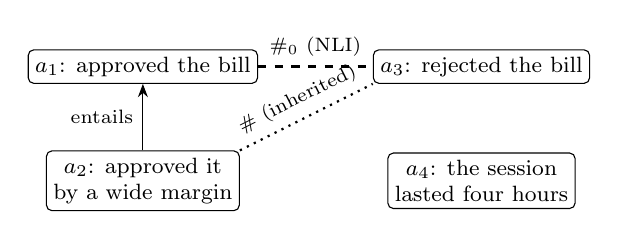
\begin{tikzpicture}[font=\footnotesize,
  cls/.style={draw, rounded corners=2pt, inner sep=2.5pt, align=center}]
  \node[cls] (a1) at (0,1.45) {$a_1$: approved the bill};
  \node[cls] (a2) at (0,0) {$a_2$: approved it\\by a wide margin};
  \node[cls] (a3) at (4.3,1.45) {$a_3$: rejected the bill};
  \node[cls] (a4) at (4.3,0) {$a_4$: the session\\lasted four hours};
  \draw[-{Stealth}] (a2) -- node[left] {\scriptsize entails} (a1);
  \draw[dashed, thick] (a1) -- node[above] {\scriptsize $\cfz$ (NLI)} (a3);
  \draw[dotted, thick] (a2.north east) -- node[above, sloped, pos=0.5] {\scriptsize $\cf$ (inherited)} (a3.south west);
\end{tikzpicture}
\caption{Worked example: worlds $\{a_1,a_2,a_4\}$ and $\{a_3,a_4\}$ with
masses $5/8$ and $3/8$; $\SE = 1.386$, $\WE = 0.662$.}
\label{fig:exemplo}
\end{subfigure}\hfill
\begin{subfigure}[b]{0.38\textwidth}\centering
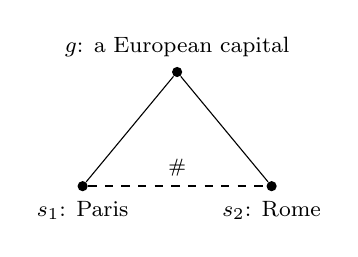
\begin{tikzpicture}[font=\footnotesize,
  dot/.style={circle, fill=black, inner sep=1.3pt}]
  \node[dot, label=above:{$g$: a European capital}] (g) at (1.2,1.45) {};
  \node[dot, label=below:{$s_1$: Paris}] (s1) at (0,0) {};
  \node[dot, label=below:{$s_2$: Rome}] (s2) at (2.4,0) {};
  \draw (s1) -- (g);
  \draw (s2) -- (g);
  \draw[dashed, thick] (s1) -- node[above] {\scriptsize $\cf$} (s2);
\end{tikzpicture}
\caption{The hedge: the core keeps only $g$ ($\SEc = 0$); the worlds are
$\{s_1,g\}$ and $\{s_2,g\}$ ($\WE = \log 2$).}
\label{fig:hedge}
\end{subfigure}
\caption{Conflict, inheritance and worlds. Solid lines are entailments (the
upper class is more general), dashed lines are contradictions reported by the
NLI model, and the dotted line is a contradiction added by inheritance.}
\label{fig:worlds}
\end{figure}

% =============================================================================
\section{What an entropy over classes cannot see}
\label{sec:blind}

\begin{observation}[Conflict blindness]
\label{obs:cegueira}
Semantic entropy, the core entropy, the number of classes, the size of the
core, the height of the order, and any other quantity computed only from the
classes, their masses and the entailment order do not change when the conflict
relation changes. In particular, for every number of classes $n \ge 2$ there
are two answer sets with $n$ classes on which all these quantities coincide,
one with a single world and one with $n$ worlds.
\end{observation}

\begin{proof}
None of these quantities takes the conflict relation as input. For the second
statement, take $n$ pairwise incomparable classes of equal mass, once with no
conflict and once with every pair in conflict. Classes, masses and order
coincide; the first set has one world, containing every class, and the second
has $n$ worlds, one for each class.
\end{proof}

The observation is immediate; its role is to state precisely what the
entailment order leaves out. Its two answer sets are not artificial. Six
answers to ``what did the hearing conclude?'' can be six compatible aspects of
one conclusion or six incompatible conclusions, and Section~\ref{sec:res-law}
shows that the first case covers most multi-class answer sets when Qwen is
asked, without the transcript, about a participant's position in a hearing,
and about half of them with Llama.
Table~\ref{tab:separacao} adds three configurations that separate the
quantities further.

\begin{table}[ht]
  \centering
  \caption{Constructed answer sets of six samples in which the quantities
  disagree (script \texttt{event\_structure}). $\SE$: semantic entropy; $\SEc$: core entropy;
  worlds and $\WE$ as in Section~\ref{sec:worlds}.}
  \label{tab:separacao}
  \small
  \begin{tabular}{@{}lcccc@{}}
    \toprule
    \textbf{Answer set} & $\SE$ & $\SEc$ & \textbf{Worlds} & $\WE$ \\
    \midrule
    Chain: one belief at six levels of detail, no conflict & 1.792 & 0.000 & 1 & 0.000 \\
    Antichain of six classes, no conflict                   & 1.792 & 1.792 & 1 & 0.000 \\
    Antichain of six classes, every pair in conflict        & 1.792 & 1.792 & 6 & 1.792 \\
    Two specific classes in conflict, each below the same &&&& \\
    \quad two general ones, plus two unrelated classes      & 1.792 & 1.792 & 2 & 0.693 \\
    Hedge: $s_1 \cf s_2$ below one general class $g$        & 1.099 & 0.000 & 2 & 0.693 \\
    \bottomrule
  \end{tabular}
\end{table}

\paragraph{The hedge.} A model that does not know an answer often hedges:
across samples it names two incompatible specifics and one safe generalisation
(``Paris'', ``Rome'', ``a European capital''). The generalisation is entailed
by both specifics, which contradict each other (Figure~\ref{fig:hedge}). Each
specific has a single class above it, so the core removes both and reports
$\SEc = 0$: no uncertainty for an answer set whose content is uncertainty. The
worlds keep the disagreement: $\{s_1, g\}$ and $\{s_2, g\}$, with
$\WE = \log 2$. This is the smallest configuration in which removing
redundancy from the order destroys the signal. Conflicts between two classes
with a common generalisation occur in $6.4\%$ of the TriviaQA answer sets,
which is consistent with the small, non-significant loss of the core entropy
against semantic entropy there (Section~\ref{sec:res-p3}).

\paragraph{The topology of conflict.} The independent sets form a simplicial
complex, the independence complex $\Ind(C^*)$ of the conflict graph
\citep{kozlov2008combinatorial}, whose maximal faces are the worlds. By
Dowker's theorem \citep{dowker1952homology}, the nerve of the cover of the
classes by worlds has the same homotopy type. Its number of connected
components $b_0$ counts blocks of classes that conflict with every class
outside their block. Its first Betti number $b_1$ can be positive only if the
consistency graph contains an induced cycle of length at least four. The
smallest example is two independent binary disagreements ($a \cf b$ and
$c \cf d$), which give four worlds and $b_1 = 1$ without any cycle of
conflicts. (An earlier draft required a cycle of five conflicting classes,
which is the smallest case only among conflict graphs that are cycles.) Our implementation reproduces the known
homotopy types of $\Ind(C_n)$ for $n = 4, \dots, 7$
\citep{kozlov2008combinatorial}. We measure $b_1 > 0$ in at most $5.8\%$ of
the answer sets of any setting and do not use it as a signal.

% =============================================================================
\section{Data and pipeline}
\label{sec:dados}

Table~\ref{tab:settings} lists the answer sets. All samples were generated by
open-weight models served with Ollama, at temperature $1.0$.

\begin{itemize}\setlength{\itemsep}{1pt}
  \item \textbf{TriviaQA, entity answers.} 233 questions from the validation
  split without context \citep{joshi2017triviaqa}, answered with only the
  entity. The label is whether a low-temperature answer ($T=0.1$) contains a
  normalised gold alias; no neural model is involved.
  \item \textbf{TriviaQA, sentence answers.} The same questions, asking for one
  complete sentence with brief context; 202 of the 233 questions have at least
  six usable sentence answers and enter the comparison. The label is the one
  of the entity answers, since the model's knowledge does not change with the
  format.
  \item \textbf{Hearing statements.} Without the transcript, the model is told
  the topic of a PublicHearingBR hearing \citep{publichearingbr} and asked, in
  one short sentence, for the position of a named participant. There is no
  usable correctness label (Section~\ref{sec:res-law}).
  \item \textbf{Nulls.} From the Qwen hearing statements: a
  \emph{half-contaminated} set keeps four of a prompt's own samples and adds
  four drawn at random from the pooled samples of all prompts, and a
  \emph{shuffled} set draws all eight from that pool.
  \item \textbf{Evidence swap.} The hearing prompt, now with five transcript
  sentences: in arm~A, the five sentences that support the gold opinion; in
  arm~B, five sentences from another, randomly drawn hearing. The answers of
  arm~B are therefore confabulated by construction: produced from evidence
  unrelated to the question.
  \item \textbf{PublicHearingBR verification.} Human-labelled opinions, each
  with the 14 transcript sentences most similar to it by embedding cosine
  \citep{reimers2019sbert} (Section~\ref{sec:neg}).
\end{itemize}

\begin{table}[ht]
  \centering
  \caption{Answer sets used in this report.}
  \label{tab:settings}
  \small
  \begin{tabular}{@{}lrrll@{}}
    \toprule
    \textbf{Setting} & \textbf{Sets} & \textbf{Samples} & \textbf{Generator} & \textbf{Label} \\
    \midrule
    TriviaQA, entity answers        & 233 & 8--10 & Qwen2.5-7B   & alias match \\
    TriviaQA, sentence answers      & 202 & 6--8  & Qwen2.5-7B   & same as entity answers \\
    Hearing statements              & 259 & 8     & Qwen2.5-7B   & --- \\
    Hearing statements              & 70  & 7--8  & Llama-3.1-8B & --- \\
    Half-contaminated and shuffled nulls & $2 \times 259$ & 8 & Qwen2.5-7B & --- \\
    Evidence swap, arms A and B     & $2 \times 80$ & 7--8 & Qwen2.5-7B & by construction \\
    PublicHearingBR verification    & 837 opinions & 14 sentences & --- & human verdict \\
    \bottomrule
  \end{tabular}
\end{table}

\paragraph{Pipeline.} For each answer set:
\begin{enumerate}\setlength{\itemsep}{1pt}
  \item run the NLI model on every ordered pair of answers, keeping the
  entailment and contradiction probabilities;
  \item threshold entailment at $0.5$, close it under transitivity, group
  mutually entailing answers into classes with masses $p$, and keep the order
  between classes;
  \item threshold contradiction at $0.5$ in either order to obtain raw
  conflict between classes;
  \item close conflict under inheritance (Definition~\ref{def:closure}) and
  set self-conflicting classes aside;
  \item enumerate the worlds (Proposition~\ref{prop:mundos}) and compute the
  number of worlds, $\WE$ and the conflict density; $\SE$ and $\SEc$ come from
  the same classes.
\end{enumerate}
No threshold was tuned: both are the values fixed in an earlier phase of the
project. The contradiction probabilities come from the same forward passes that
semantic entropy needs for entailment, so worlds add no model calls.

\paragraph{Statistics.} On TriviaQA each question is scored by its negated
uncertainty, and the AUROC measures how well the score predicts that the
answer is correct; ties count one half. Differences are point estimates. Their
$95\%$ intervals are the $2.5$ and $97.5$ percentiles of $5{,}000$ bootstrap
resamples of the unit named in the text: questions for TriviaQA (paired
between the two scores), prompts for the evidence swap, and hearings for
PublicHearingBR, whose opinions from the same hearing are not independent.
Proportions carry Wilson intervals.

% =============================================================================
\section{Results on answer sets}
\label{sec:res}

\subsection{Conflict carries information the order does not}
\label{sec:res-tqa}

On TriviaQA, contradiction fires on $30.0\%$ of the unordered pairs of samples.
Of the class pairs in conflict, $97.9\%$ are incomparable in the entailment
order, so conflict is not a restatement of the order. The NLI model almost
satisfies inheritance by itself (mean closure cost $0.81\%$ of class pairs per
answer set) and rarely produces self-conflicting classes (on average $1.67\%$
of the classes of an answer set). In all, $55.4\%$ of the
answer sets contain at least one conflict and $53.6\%$ have more than one world
($2.63$ worlds on average).

The conflict relation means what its name says. We check this without any
neural model, by matching each individual sample against the gold aliases:
pairs of samples in conflict differ in correctness (one matches, the other does
not) in $21.0\%$ of cases, against $4.0\%$ for pairs not in conflict
(difference $+0.170$, $95\%$ CI $[+0.113, +0.229]$, resampling questions).

Table~\ref{tab:estratos} splits the questions by the kind of diversity among
their samples. Semantic entropy treats the two lower rows as the same kind of
evidence, differing only in amount. Accuracy falls across the three rows. The
fall from one class to several classes in one world is significant
($+0.367$ $[+0.122, +0.600]$); the fall from one world to several
($+0.220$ $[-0.018, +0.459]$) rests on only 18 one-world sets, and its
interval includes zero. Correct answers come from sets with $1.61$
worlds on average, wrong answers from sets with $3.53$.

\begin{table}[ht]
  \centering
  \caption{Accuracy of the model's answer by kind of diversity among its
  samples (TriviaQA, entity answers). Means of $\SE$ and $\WE$ per stratum.}
  \label{tab:estratos}
  \small
  \begin{tabular}{@{}lrccc@{}}
    \toprule
    \textbf{Stratum} & $n$ & \textbf{Accuracy} [$95\%$ CI] & $\SE$ & $\WE$ \\
    \midrule
    One class                          & 90  & $81.1\%$ [$71.8$, $87.9$] & 0.000 & 0.000 \\
    Several classes, one world         & 18  & $44.4\%$ [$24.6$, $66.3$] & 0.626 & 0.000 \\
    Several classes, several worlds    & 125 & $22.4\%$ [$16.0$, $30.5$] & 1.300 & 1.103 \\
    \bottomrule
  \end{tabular}
\end{table}

\subsection{Worlds do not outperform semantic entropy where it works}
\label{sec:res-p3}

Table~\ref{tab:tqa} compares the scores as detectors of wrong answers. Semantic
entropy reaches $0.811$, reproducing the value of the earlier phase from the
same cached samples (prediction P1). Neither order-aware nor conflict-aware
corrections improve on it. The registered primary comparison, $\WE$ against
$\SE$, gives $-0.0191$ $[-0.0445, +0.0057]$ (P3, not confirmed), and $\WE$
does no better than the core entropy ($-0.0043$ $[-0.0277, +0.0185]$). $\WE$
does not outperform the scalar conflict density either ($+0.0221$
$[-0.0187, +0.0646]$; P4, not confirmed), and adding it to the density by rank
sum, the other arm of P4, which we ran only on 30 September 2026, gives
$+0.0203$ $[-0.0027, +0.0451]$. Counting classes ($0.809$) is as good as any
refinement. The conflation rate suggests why: on TriviaQA only $12.6\%$ of the multi-class
answer sets form a single world ($9.8\%$ contain no contradiction at all), so
the classes semantic entropy counts are nearly always disagreements, and a
conflict-aware score has little to correct.

\begin{table}[ht]
  \centering
  \caption{Detecting wrong answers on TriviaQA ($n=233$, accuracy $46.8\%$).
  Left: AUROC. Right: paired differences with $95\%$ intervals. LGU is our
  reimplementation of \citet{lgu2026logical} from its description.}
  \label{tab:tqa}
  \small
  \begin{tabular}{@{}lc@{\hspace{2.2em}}lc@{}}
    \toprule
    \textbf{Score} & \textbf{AUROC} & \textbf{Comparison} & $\Delta$ \textbf{AUROC} [$95\%$ CI] \\
    \midrule
    Semantic entropy $\SE$   & 0.811 & $\WE - \SE$ (P3)          & $-0.0191$ [$-0.0445$, $+0.0057$] \\
    Number of classes        & 0.809 & $\SEc - \SE$              & $-0.0148$ [$-0.0358$, $+0.0030$] \\
    LGU                      & 0.805 & $\WE - \SEc$              & $-0.0043$ [$-0.0277$, $+0.0185$] \\
    Core entropy $\SEc$      & 0.796 & $\WE -{}$conflict density (P4) & $+0.0221$ [$-0.0187$, $+0.0646$] \\
    World entropy $\WE$      & 0.792 & worlds${}-{}$conflict density  & $+0.0214$ [$-0.0191$, $+0.0625$] \\
    Number of worlds         & 0.791 & $\WE - $LGU               & $-0.0135$ [$-0.0329$, $+0.0040$] \\
    Conflict density         & 0.770 &                           & \\
    \bottomrule
  \end{tabular}
\end{table}

\subsection{The conflation rate varies across settings}
\label{sec:res-law}

Table~\ref{tab:conflacao} applies the same code, NLI model and thresholds to
the hearing statements and to the two nulls. The number of classes, worlds,
entropies and densities are means over answer sets, which is why they are not
integers.

\begin{table}[ht]
  \centering
  \caption{Conflict structure by setting (scripts \texttt{domain\_conflict} and \texttt{intervals}).
  Means over answer sets, except $n$ and the conflation rate, which is the
  share of multi-class sets forming a single world (Wilson $95\%$ interval).}
  \label{tab:conflacao}
  \small
  \setlength{\tabcolsep}{4pt}
  \begin{tabular}{@{}lrrrrrrrr@{}}
    \toprule
    \textbf{Setting} & $n$ & \textbf{Classes} & \textbf{Worlds} & $>$\textbf{1 world} & $\SE$ & $\WE$ & \textbf{Density} & \textbf{Conflation} \\
    \midrule
    Hearing statements, Qwen  & 259 & 4.14 & 1.23 & $18.5\%$ & 1.112 & 0.125 & 0.103 & $\mathbf{78.5\%}$ [$72.6$, $83.4$] \\
    Hearing statements, Llama & 70  & 6.11 & 1.87 & $50.0\%$ & 1.644 & 0.393 & 0.230 & $49.3\%$ [$37.8$, $60.8$] \\
    TriviaQA, entity answers  & 233 & 3.28 & 2.63 & $53.6\%$ & 0.746 & 0.592 & 0.473 & $\mathbf{12.6\%}$ [$8.1$, $19.0$] \\
    Half-contaminated null    & 259 & 6.65 & 2.97 & $94.2\%$ & 1.800 & 0.933 & 0.424 & $5.8\%$ [$3.5$, $9.3$] \\
    Shuffled null             & 259 & 7.91 & 4.06 & $98.5\%$ & 2.063 & 1.288 & 0.423 & $1.5\%$ [$0.6$, $3.9$] \\
    \bottomrule
  \end{tabular}
\end{table}

We read the table in three steps. First, when the model is asked about a
participant's position without the transcript, $78.5\%$ of the answer sets
with several classes form a single world: the diversity that semantic entropy
measures there (mean $1.112$) is mostly elaboration and complementary detail,
and the world entropy is about nine times lower ($0.125$). On TriviaQA the
share is $12.6\%$. The Llama replication lies in between ($49.3\%$), with
more varied samples ($6.11$ classes per set against $4.14$). A few of the
one-world sets do contain a contradiction involving a self-conflicting class
(15 of 175 for Qwen, 3 of 34 for Llama, 4 of 18 on TriviaQA); counting only
sets with no contradiction at all gives $71.7\%$, $44.9\%$ and $9.8\%$, in
the same order.
Second, the nulls behave as contamination should: replacing a prompt's
samples by samples drawn from the pool raises the number of worlds
monotonically ($1.23$, $2.97$, $4.06$). Where the conflict density saturates ($0.424$ and
$0.423$), the number of worlds still separates the two nulls, so it carries
information that the density does not. We had predicted that unrelated statements would rarely
contradict each other and that the shuffled null would stay near one world
(P7); instead, the NLI model reads many statements from different hearings as
contradictory, such as two statements that name different states as
recipients. Third, the diagnostics stay small: in the hearing settings, nulls
and evidence-swap arms, the mean closure cost per answer set is $2.2$ to
$6.0\%$ of class pairs and the mean self-conflict rate $3.2$ to $5.5\%$ of
classes (on TriviaQA, $0.81\%$ and $1.67\%$).

In our research log this pattern was called the \emph{conflation law}: semantic
entropy works where the diversity it counts is disagreement. The table alone
cannot establish it, because the hearing statements offer no working
reference: without the transcript the model almost never knows the answer,
correctness hardly varies, and in an earlier phase of the project every score
we tried there, semantic entropy included, was at chance. With one labelled
setting, the conflation rate is a hypothesis about the scope of semantic
entropy, which we test by intervention.

\subsection{Raising the conflation rate lowers the AUROC of semantic entropy}
\label{sec:res-h5}

If semantic entropy works where the diversity it measures is disagreement,
changing only the form of the answers should move both. We asked the same
TriviaQA questions for a complete sentence with brief context instead of a bare
entity, keeping the label of the entity answers. Four predictions were
registered in the script before the analysis (Section~\ref{sec:pred}).

\begin{table}[ht]
  \centering
  \caption{The same 202 TriviaQA questions and labels, answered with an entity
  or with a sentence (scripts \texttt{conflation\_intervention} and \texttt{intervals}). Rows above the
  line are means over answer sets, except the conflation rate. Differences are
  paired over questions.}
  \label{tab:h5}
  \small
  \begin{tabular}{@{}lccc@{}}
    \toprule
     & \textbf{Entity} & \textbf{Sentence} & \textbf{Sentence $-$ entity} [$95\%$ CI] \\
    \midrule
    Classes                    & 3.57     & 4.24     & \\
    Worlds                     & 2.84     & 2.63     & \\
    Semantic entropy $\SE$     & 0.840    & 1.106    & \\
    World entropy $\WE$        & 0.667    & 0.645    & \\
    Conflation rate            & $12.6\%$ & $29.0\%$ & $+0.164$ [$+0.077$, $+0.250$] \\
    \midrule
    AUROC of $\SE$             & 0.816    & 0.721    & $-0.0953$ [$-0.1746$, $-0.0157$] \\
    AUROC of $\WE$             & 0.794    & 0.751    & $-0.0435$ [$-0.1187$, $+0.0270$] \\
    AUROC of $\SEc$            & 0.801    & 0.765    & \\
    \bottomrule
  \end{tabular}
\end{table}

With sentence answers the conflation rate more than doubles, from $12.6\%$ to
$29.0\%$ ($+0.164$ $[+0.077, +0.250]$; $9.6\%$ to $24.3\%$ counting only sets
with no contradiction at all), less than the $40\%$ we had predicted, and the
AUROC of semantic entropy falls from $0.816$ to $0.721$ ($-0.0953$
$[-0.1746, -0.0157]$; Table~\ref{tab:h5}). This is the one comparison in this
report in which a change predicted from the conflation rate is observed on
labelled data, with questions and labels held fixed. The sentence answers
have at most eight samples per question, against ten for entity answers;
restricting the entity answers to their first eight samples leaves semantic
entropy at $0.819$ and the drop at $-0.0985$ $[-0.1756, -0.0192]$, so the
smaller sample does not explain it. The world entropy falls less and ends
above semantic entropy ($0.751$ against $0.721$), but neither the difference
between the two scores ($+0.0302$ $[-0.0219, +0.0837]$) nor the difference
between their drops ($-0.0518$ $[-0.1096, +0.0044]$) is significant. The core
entropy also falls less and reaches $0.765$, the highest of the three with
sentence answers; we had not registered this comparison and report it as an
observation ($\WE - \SEc = -0.0136$ $[-0.0529, +0.0269]$). The sentence
answers still carry the entity: a gold alias appears in $47.7\%$ of them, and
the per-question share of such answers correlates with the label at $+0.692$.

% =============================================================================
\section{Negative results}
\label{sec:neg}

\paragraph{Contradictions in the evidence do not indicate hallucination.} The
main paper's task is to decide whether an opinion attributed to a participant
is supported by the transcript. The consistency structure can be carried to
that task only through the evidence. For an opinion, take the 14 transcript
sentences most similar to it and keep those that entail it with probability at
least $0.35$ (its \emph{support}); order them by entailment and relate them by
contradiction as in Section~\ref{sec:worlds}, with equal masses. We predicted
(P8) that an opinion whose support spans two or more worlds, that is, support
that cannot all be true, would more often be unsupported. We tested this on the
837 opinions from 40 hearings for which these features were computed (93 of
them unsupported). The prediction fails (Table~\ref{tab:h4}): the number of
worlds in the support, its world entropy and the flag for support spanning
several worlds all score below chance, with intervals that resample hearings
and exclude $0.5$. The reason is the size of the support. An opinion with no
supporting sentence ($21.6\%$ of them) has no world at all, the number of
worlds grows with the number of supporting sentences (correlation $+0.69$),
and opinions with more support are less often unsupported (support size alone
scores $0.602$). Among the 495 opinions with at least two supporting
sentences (44 unsupported), comparing only opinions with the same number of
supporting sentences, the number of worlds scores $0.512$ $[0.456, 0.571]$;
its entropy gives the same value and the flag $0.510$ $[0.455, 0.568]$. We
detect no information in the coherence of the evidence beyond its amount. A
plausible reading is that well-discussed opinions attract more evidence and,
with it, more contradictions. Contradiction between the opinion
and any retrieved sentence is at chance.

\begin{table}[ht]
  \centering
  \caption{Consistency features against the human verdict in PublicHearingBR
  ($n=837$ opinions from 40 hearings, 93 unsupported; scripts \texttt{incoherent\_support} and
  \texttt{intervals}). AUROC for detecting unsupported opinions, with $95\%$ intervals
  that resample hearings.}
  \label{tab:h4}
  \small
  \begin{tabular}{@{}lcc@{}}
    \toprule
    \textbf{Feature} & \textbf{AUROC} & [$95\%$ CI] \\
    \midrule
    Maximum entailment of the opinion (baseline)  & 0.598 & [0.527, 0.676] \\
    Size of the support (threshold $0.35$)         & 0.602 & [0.542, 0.665] \\
    Maximum embedding cosine                       & 0.544 & [0.451, 0.645] \\
    Contradiction between opinion and evidence     & 0.504 & [0.428, 0.580] \\
    World entropy of the support                   & 0.459 & [0.424, 0.497] \\
    Support spans several worlds (flag)            & 0.457 & [0.424, 0.494] \\
    Number of worlds in the support                & 0.433 & [0.374, 0.489] \\
    \bottomrule
  \end{tabular}
\end{table}

\paragraph{None of the self-consistency quantities we tested detects answers
built on misleading evidence.} In the evidence swap, the answers of arm~B share $20$ times less
vocabulary with the gold opinion than those of arm~A (Jaccard overlap of
content words $0.008$ against $0.167$; paired difference $+0.159$
$[+0.132, +0.185]$), so they are confabulated. As registered (P6), no quantity
separates the arms (paired differences A$-$B over the 80 prompts): number of
worlds $+0.138$ $[-0.037, +0.325]$, world entropy $+0.080$ $[-0.015, +0.172]$,
conflict density $-0.009$ $[-0.089, +0.068]$, semantic entropy $+0.012$
$[-0.160, +0.184]$. As far as these measures can tell, a model given the wrong
evidence answers as consistently as one given the right evidence; we found no
quantity, with or without worlds, that separates the two.

% =============================================================================
\section{Predictions and outcomes}
\label{sec:pred}

Predictions P1--P8 were registered on 3 August 2026, before any AUROC of the
new quantities was computed; P3 and P4
were the confirmatory comparisons, and the rest were secondary or
exploratory. The predictions for the sentence-answer intervention were
registered in the header of \texttt{conflation\_intervention} before its analysis.
Table~\ref{tab:pred} lists every outcome.

\begin{table}[ht]
  \centering
  \caption{Registered predictions and their outcomes. $^*$Confirmatory.}
  \label{tab:pred}
  \small
  \begin{tabular}{@{}l>{\raggedright\arraybackslash}p{6.2cm}>{\raggedright\arraybackslash}p{5.7cm}@{}}
    \toprule
    & \textbf{Prediction} & \textbf{Outcome} \\
    \midrule
    P1 & $\SE$ reproduces $0.811$ from the cached samples & Confirmed ($0.811$) \\
    P2 & Most conflicts join incomparable classes; closure cost below $10\%$; self-conflict below $5\%$ & Confirmed ($97.9\%$; $0.81\%$; $1.67\%$) \\
    P3$^*$ & $\WE$ loses less to $\SE$ than $\SEc$ does ($-0.0149$); hoped for $\WE \ge \SE$ & Not confirmed ($-0.0191$ [$-0.0445$, $+0.0057$]) \\
    P4$^*$ & Worlds or $\WE$ outperform the conflict density, or add to it in combination & Not confirmed ($+0.0221$ [$-0.0187$, $+0.0646$]; combination $+0.0203$ [$-0.0027$, $+0.0451$], run late) \\
    P5 & Among the 28 answer sets with redundant classes (core smaller than the class count), wrong answers have more worlds (exploratory) & Direction as predicted, not significant (AUROC of worlds $0.655$ [$0.417$, $0.873$]) \\
    P6 & No world quantity separates the evidence-swap arms & Confirmed (Section~\ref{sec:neg}) \\
    P7 & Hearing statements mostly form one world; so does the shuffled null & First half confirmed ($81.5\%$ of sets); second refuted ($4.06$ worlds) \\
    P8 & Support spanning several worlds concentrates hallucinations & Refuted: below chance ($0.43$--$0.46$) through support size; $0.512$ [$0.456$, $0.571$] at equal size \\
    \midrule
    h5 (i) & Conflation rises to at least $40\%$ with sentence answers & Not confirmed: it rises ($+0.164$ [$+0.077$, $+0.250$]), but to $29.0\%$ [$22.7$, $36.2$] \\
    h5 (ii) & The AUROC of $\SE$ falls with sentence answers & Confirmed ($-0.0953$ [$-0.1746$, $-0.0157$]) \\
    h5 (iii) & $\WE \ge \SE$ with sentence answers & Not significant ($+0.0302$ [$-0.0219$, $+0.0837$]) \\
    h5 (iv) & $\SE$ falls more than $\WE$ & Direction as predicted, not significant ($-0.0518$ [$-0.1096$, $+0.0044$]) \\
    \bottomrule
  \end{tabular}
\end{table}

% =============================================================================
\section{Limitations}
\label{sec:lim}

\emph{One verifier.} Every relation in this report comes from one multilingual
NLI checkpoint at fixed thresholds. The conflict relation is only as good as
that model; the nulls show that it reads many unrelated hearing statements as
contradictory, and we report closure cost and self-conflict rather than hide
them.

\emph{Few generators and settings.} Two small open models (Qwen2.5-7B and
Llama-3.1-8B), one question-answering benchmark and one task on hearings. The
conflation rate is a property of a combination of model, prompt and domain,
and the Llama replication already moves it from $78.5\%$ to $49.3\%$. More
generators and domains are needed before the pattern can be called general.

\emph{Labels and causality.} Only TriviaQA has correctness labels, and they
come from alias matching. The evidence that the conflation rate governs the
AUROC of semantic entropy rests on a single intervention with 202 questions,
which changes the format of the answers and, with it, possibly other
properties of the samples; within it, the advantage of world entropy is not
significant. No comparison was corrected for multiplicity: P3 and P4 were
designated as confirmatory in advance, and every other comparison should be
read as exploratory.

\emph{Scope of the verification test.} The PublicHearingBR analysis covers the
837 opinions of an earlier, interrupted collection, not the $3{,}630$ opinions
of the main paper, and uses the 14 most similar sentences rather than the
attributed speaker's turns.

\emph{Comparators.} The core entropy is our own construction, and LGU is a
reimplementation from its description; neither is an official
implementation.

\emph{A corrected script.} While preparing this report we found that the
script for Table~\ref{tab:conflacao} treated two identical samples as
different classes. The corrected values are reported. The correction affects
the settings with repeated samples (the Qwen hearing statements, the
half-contaminated null and the evidence-swap arms): it lowers their mean
number of classes and $\SE$ (for Qwen, from the previously reported $4.31$ and
$1.151$ to $4.14$ and $1.112$), changes their conflict densities, verifier
diagnostics and evidence-swap differences slightly, leaves the numbers of
worlds and $\WE$ unchanged, and moves the conflation rates by at most $0.4$
percentage points.

% =============================================================================
\section{Conclusion}
\label{sec:conc}

Semantic entropy counts how many different meanings a model produces, but not
whether those meanings exclude one another. The contradiction probabilities
that the NLI model already computes are enough to tell the two apart: once
conflict is inherited along entailment, the maximal consistent subsets of an
answer set are its maximal independent sets, which a standard clique algorithm
enumerates exactly. On TriviaQA, where almost all diversity among answers is
disagreement, the distinction adds nothing to semantic entropy as a detector,
but it helps explain why semantic entropy works there. When Qwen states the
positions of hearing participants without the transcript, most multi-class
answer sets form a single world (about half with Llama), and asking TriviaQA
questions for full sentences both raises the share of such sets and lowers
the AUROC of semantic entropy. Because the conflation rate needs no labels, it can be
measured in a new setting before an uncertainty method is trusted there. Our
results do not show that world entropy should replace semantic entropy, and
they do not carry over to the verification task of the main paper, where we
detect no information in the contradictions within the evidence beyond its
amount.

\medskip\noindent\textbf{Reproducibility.} The directory \texttt{code/}
next to this report's directory contains every script and cached intermediate
result, and \texttt{code/run\_all.sh} runs them. The scripts
\texttt{event\_structure}, \texttt{triviaqa\_worlds}, \texttt{domain\_conflict},
\texttt{conflation\_intervention} and \texttt{intervals} run offline in about a
minute on a laptop and print every number in this report;
\texttt{incoherent\_support} also needs the PublicHearingBR data, as in the main
repository. No language model or NLI call is needed unless the caches are
deleted. \texttt{README.md} lists the commands and the expected output.

\begingroup
\footnotesize
\setlength{\bibsep}{0pt plus 0.2ex}
\bibliography{references}
\endgroup

\end{document}
